\chapter{Разработка алгоритмов и средств динамической идентификации}
%TODO
 
\section{Описание исследуемого объекта}
%TODO: Добавить описание котельного агрегата, базы данных

\section{Выбор архитектуры нейронных сетей}

Появление методов глубокого обучения привели к появлекнию множества различных архитектур нейронных сетей, в частности их компонентов. Архитектура нейронной сети во многом определяется классом задачи и её правильный выбор необходимо делать исходя из особенностей данных и желаемого результата. Несмотря на широкий спектр задач, которые решают те или иные архитектуры, не все модели подходят для решения задач идентификации.

\subsection{Полносвязная нейронная сеть}

Полносвязанные нейронные сети — это нейронные сети, в которых каждый 
нейрон передает свой выходной сигнал остальным нейронам, в том числе 
и самому себе. 

\begin{figure}[htbp]
  \centering
    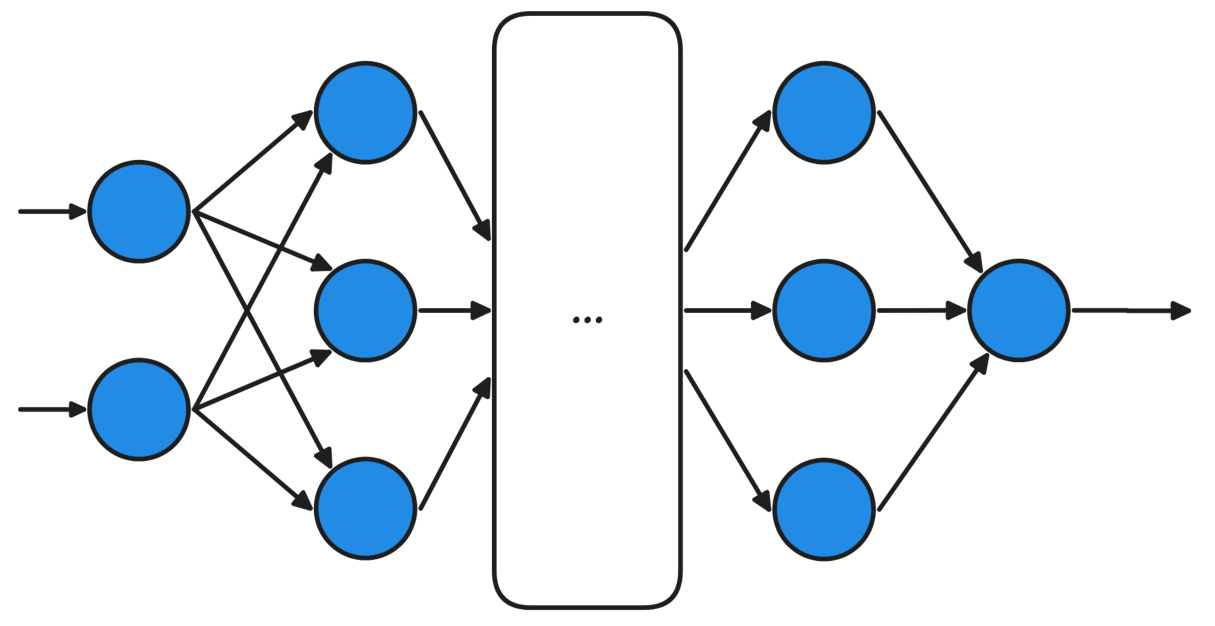
\includegraphics[width=0.9\textwidth]{figures/arch_fully_connected.png}
  \caption{Архитектура полносвязной сети}\label{fig:dense_nn}
\end{figure}

Все входные сигналы подаются всем нейронам, находящимся 
на текущем слое (см. рис. \ref{fig:dense_nn}). Выходными сигналами сети могут быть все или некоторые
выходные сигналы нейронов.

Такие модели могут использоваться для аппроксимации сложных многомерных
функций, представляющих множество целей оптимизации. Часто применяются для
построения суррогатных моделей для оценки функций без необходимости прямого
вычисления.

\subsection{Рекуррентная нейронная сеть}

Рекуррентная нейронная сеть — это тип искусственных нейронных сетей, широко
используемый для обработки последовательных данных и временных рядов. 

\begin{figure}[htbp]
  \centering
    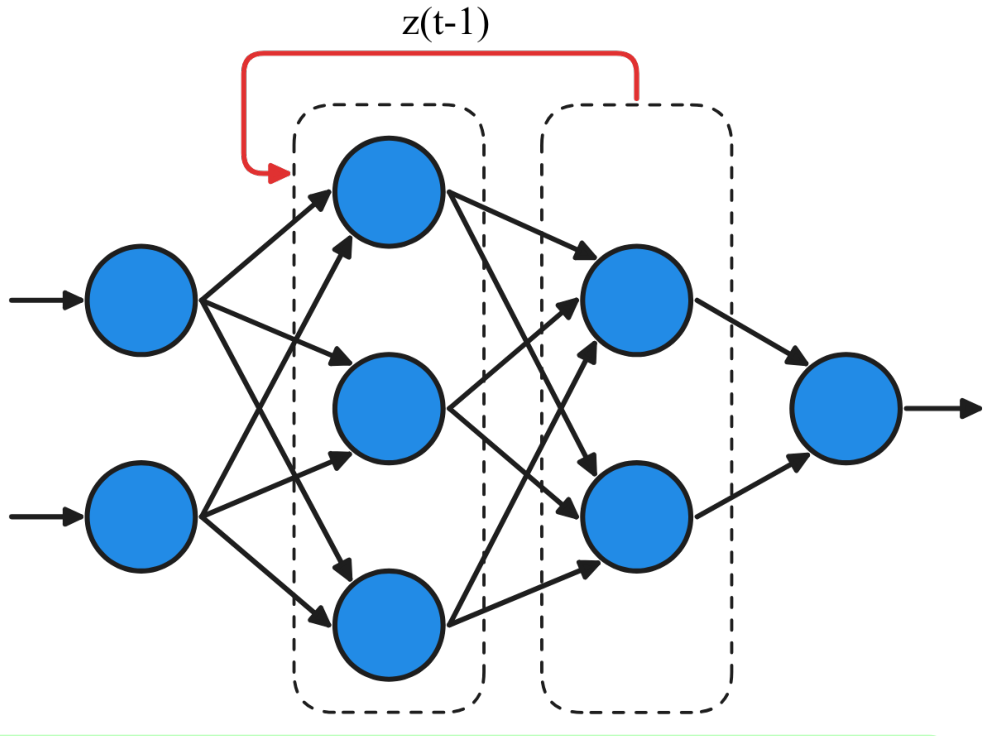
\includegraphics[width=0.9\textwidth]{figures/arch_rnn.png}
  \caption{Архитектура рекуррентной сети}\label{fig:rnn}
\end{figure}

В отличие от традиционных нейронных сетей, например, многослойных перцептронов, где
обработка данных происходит только в одном направлении, RNN имеют петли (см.
рис. \ref{fig:rnn}). Эти петли позволяют сохранять и использовать информацию из 
предыдущих состояний сети, что делает RNN особенно полезными для задач, где важен 
контекст и зависимость данных во времени. 

В задачах динамической идентификации, где необходимо учитывать не только прямые
связи систем, но также и краевые эффекты, оказывающие влияние на смежные
системы, RNN могут быть полезны благодаря своей способности учитывать контекст
и исторические данные.

\subsection{Сверточная нейронная сеть}

Сверточная нейронная сеть — особый тип нейронной сети, основанный на
полносвязной сети и имеющий как минимум один особый сверточный слой. 

\begin{figure}[htbp]
  \centering
    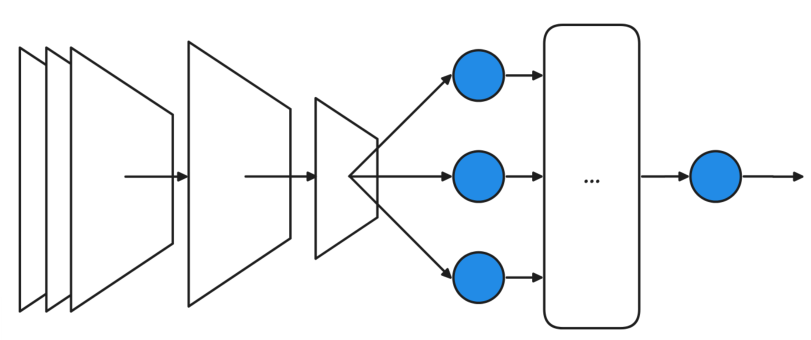
\includegraphics[width=0.9\textwidth]{figures/arch_cnn.png}
  \caption{Архитектура сверточной сети}\label{fig:cnn}
\end{figure}

Сверточный слой — нейронный слой, позволяющий производить понижение или повышение
размерности данных. Из-за своей особой архитектуры (см. рис. \ref{fig:cnn}),
сети позволяют эффективно обрабатывать данные с пространственной структурой.

Данная категория нейронных сетей применяется в случаях, если входы системы
имеют пространственную структуру, в которой элементы связанны между собой. Они
применяются для обнаружения признаков или шаблонов, влияющих на общую работу
системы.

Зачастую данный тип нейронных сетей используется в связи с другими
архитектурами, предоставляя им возможности работы с небольшими данными с
выделенными общими признаками.

\subsection{Автокодировочная нейронная сеть}

Автокодировщик — это тип нейронной сети, используемой для обучения эффективного
кодирования данных. Цель автокодировщика — научиться представлять входные
данные в более сжатом и информативном виде, называемом латентным пространством,
и затем восстанавливать оригинальные данные из этого представления. 
\begin{figure}[htbp]
  \centering
    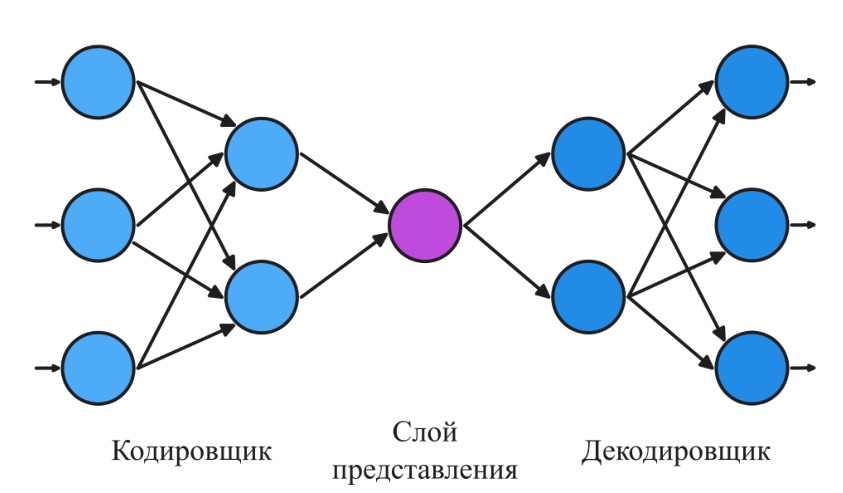
\includegraphics[width=0.9\textwidth]{figures/arch_autoencoder.png}
  \caption{Архитектура сети-автокодировщика}\label{fig:autoencoder_nn}
\end{figure}

Он состоит из двух основных частей: энкодера и декодера (см. рис.
\ref{fig:autoencoder_nn}). Энкодер преобразует входные данные в сжатое 
скрытое представление (латентное пространство), а декодер восстанавливает 
исходные данные из этого представления. Задача декодера — восстановить данные 
из их скрытого сжатого представления. Данный тип моделей позволяет находить 
компактные представления данных и выявлять скрытые закономерности в них.
В некоторых типах автокодировщиков добавляют вероятностную интерпретацию, что
позволяет моделировать неопределенности в данных и оптимизировать несколько
целей одновременно через латентное пространство.

Архитектурные особенности автокодировщиков не предполагают использования их в
качестве моделей, описывающих системы, однако могут использоваться с целью
повторения помех в данных и приближения их к реальным.

\subsection{Сравнение архитектур}

\section{Декомпозиционный метод идентификации нейронными сетями}
%TODO: Описание предлагаемого метода

\section{Программное обеспечение динамической идентификации}
%TODO: Привести информацию о наличии других ПО для моделирования
%       и то, что зачастую сложные методы поставляются с использованием замкнутого цикла ПО

\subsection{Требования к системе}
%TODO: Привести требования к предлагаемому ПО

\subsection{Структуры данных}
%TODO: Какие структуры данных, их иерархия, паттерны использовались

\subsection{Архитектура приложения}
%TODO: Привести список компонентов, их назначение и связь между собой

\subsection{Используемые формы}
%TODO: Перечисление форм и их назначение, какие возможности предоставляют

\subsection{Работа с приложением}
%TODO: Описать как работать с приложением и какие возможности оно предоставляет

\section{Архитектура связей нейронных сетей}
%TODO: Описать какие модели используются при обучении для описания каждой подсистемы и системы в общем

\section{Оценка работы}
%TODO: Произвести оценку моделирования системы
